\documentclass[cn]{elegantbook}
<<<<<<< HEAD
\usepackage[ruled, vlined]{algorithm2e}
=======
\usepackage[ruled,vlined]{algorithm2e}
\usepackage{algorithmicx}
\usepackage{algpseudocodex}
\usepackage{amsmath}
>>>>>>> temp

\title{何老师算法课笔记}
\subtitle{还没有想好的副标题}
\author{计卓1801全体}
\institute{华中科技大学}
\date{\zhtoday}
\version{1.0.0}
\logo{logo.png}
\cover{cover.png}

\begin{document}
\maketitle
\tableofcontents
  \maketitle
  \tableofcontents

  % add your code here
  \chapter{分治算法之平面最近点对问题}

\begin{introduction}
\item 平面最近点对问题定义
\item 分治算法设计
\item 分治算法时间复杂度分析
\item 伪代码
\end{introduction}

\section{平面最近点对问题定义}
给定二维平面上的$n(n \ge 2)$个不同的点$p$组成点集$P = \{p_i \big| 1\le i \le n\}$,
设计算法寻找欧式距离最近的点对$(A,B)$。
\begin{figure}[htb]
    \centering
    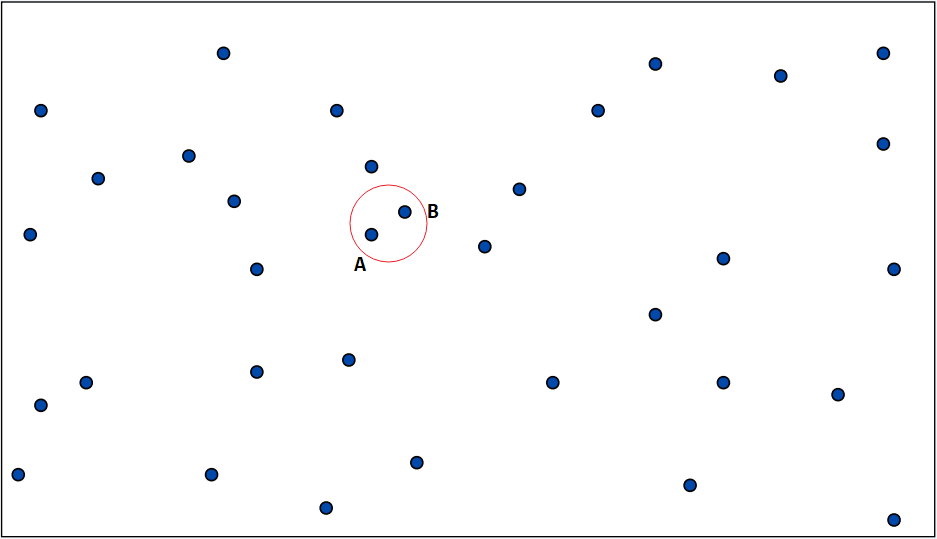
\includegraphics[scale=0.5]{Ln9.image/NearestPointsDef.png}
    \caption{问题定义图例}\label{fig1}
\end{figure}

如上图\autoref{fig1}中点对$(A,B)$即为问题的答案。

\section{分治算法设计}
对于这样一个问题,我们很直接地可以使用BF (Brute Force)算法进行暴力求解,
即二重循环计算所有点之间的距离,从而获得最小距离,显然该算法的时间复杂度为
$O(n^2)$。那么有没有更快的算法呢?本章我们使用经典的算法思想——分治,
设计一个$O(n\log n)$的算法。

\subsection{分治问题}
遵循分治思想,我们首先要考虑如何分治问题使得问题规模约减。

我们使用X坐标作为第一关键字、Y坐标作为第二关键字,对点集$P$进行排序,
并以点$p_{\lfloor\frac{n}{2}\rfloor}$作为分治点,获得如下两个点集:
\begin{equation*}
    P_1 = \{p_i\ \big|\ 1 \le i \le \lfloor\frac{n}{2}\rfloor \}
\end{equation*}
\begin{equation*}
    P_2 = \{p_i\ \big|\ \lfloor\frac{n}{2}\rfloor < i \le n\}
\end{equation*}
这样就将当前问题约减为两个规模为$\frac{n}{2}$的子问题
分治过程如\autoref{fig2}中所示。

\begin{figure}[htb]
    \centering
    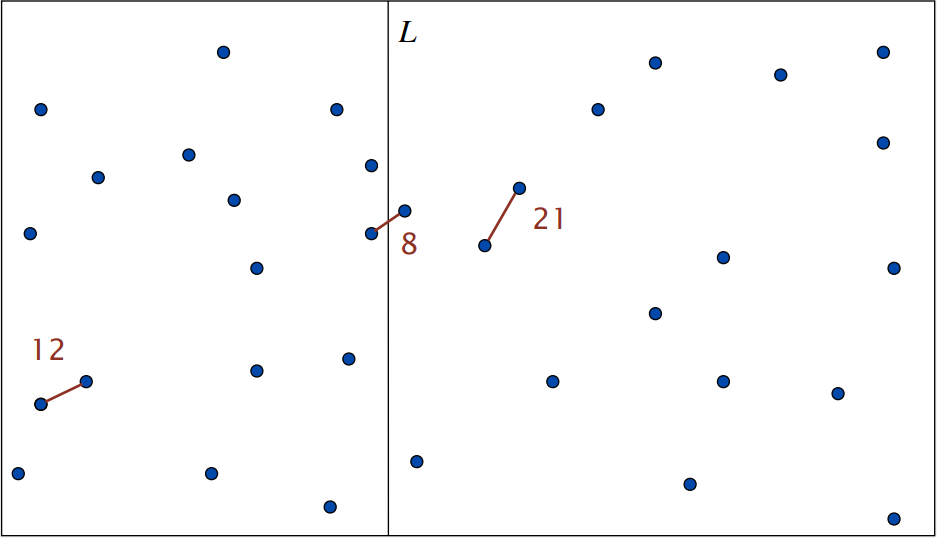
\includegraphics[scale=0.5]{Ln9.image/NearestPointsDivide.png}
    \caption{分治过程图例}\label{fig2}
\end{figure}

如此递归下去,我们可以求得两个点集相对应的最近点对距离$\delta_1, \delta_2$,取其中较小值
记为$\delta = \min \{ \delta_1 , \delta_2 \}$。

当分治到点集大小为2个或3个时,可以在常数时间内计算出子问题的解。

\subsection{合并结果}

接着,我们需要考虑如何合并子问题的解。

上述的$\delta$一定是正确的合并结果嘛?显然不是,我们并没有考虑,一端在$P_1$,
一端在$P_2$的线段。因此,在合并阶段,我们要将这种情况考虑在内。

这里,我们将所有横坐标与分治点$p_{\lfloor\frac{n}{2}\rfloor}$的横坐标
$x_{\lfloor\frac{n}{2}\rfloor}$差值小于$\delta$的点组成集合$B$,即
\begin{equation*}
    B = \{p_i\ \big|\ 
        \left|x_i - x_{\lfloor\frac{n}{2}\rfloor}\right| \le \delta ,\
        1 \le i \le n\}
\end{equation*}   
因为只有$B$集合中的点之间的距离才有可能小于$\delta$。
$B$集合如下图\autoref{fig3}中阴影部分所示:
\begin{figure}[htb]
    \centering
    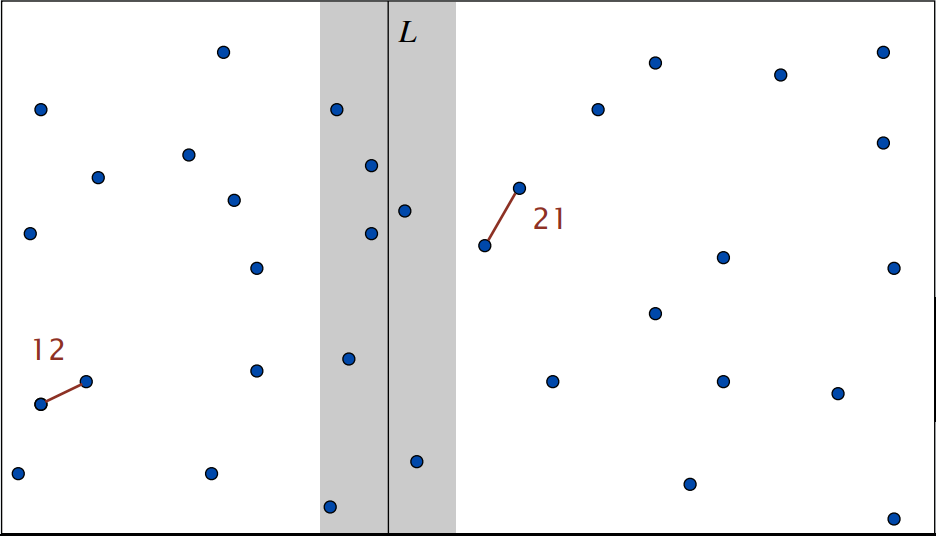
\includegraphics[scale=0.5]{Ln9.image/NearestPointsMerge.png}
    \caption{合并过程图例}\label{fig3}
\end{figure}

进一步,我们的目标是检验在$B$集合中是否存在距离比$\delta$更近的点对,以此更新当前问题的解
。因此,对于每个$p_i = (x_i, y_i) \in B$遍历所有在其之下竖直距离不超过$\delta$的点,
即遍历集合
\begin{equation*}
    C(p_i) = \{ p_j\ \big|\ y_i - \delta \le y_j \le y_i, p_j \in B \}
\end{equation*}
为了方便遍历,我们可能会想到对$B$集合中的点,以Y坐标为第一关键字,X坐标为第二关键字,进行排序。
但是如此一来,每一次合并的时间复杂度为$O(n \log n)$,徒增时间消耗,因此我们采取合并策略,即
按照Y坐标为关键字,进行$P_1, P_2$的归并来直接获得排序后的集合$B$,这样只需要$O(n)$的时间。

考虑到$C(p_i)$会因为归并操作而维持在$O(n)$数量级,其实不然,该集合的大小不会超过7。下面给出
证明。

根据定义,$C(p_i)$中的点的纵坐标均处于$(y_i - \delta, y_i]$范围内,且其中的所有点
的横坐标均处于$\left( x_m - \delta, x_m + \delta \right)$范围内。
这样便构成了一个$2\delta\times\delta$的矩形。如下图\autoref{fig4}所示
\begin{figure}[htb]
    \centering
    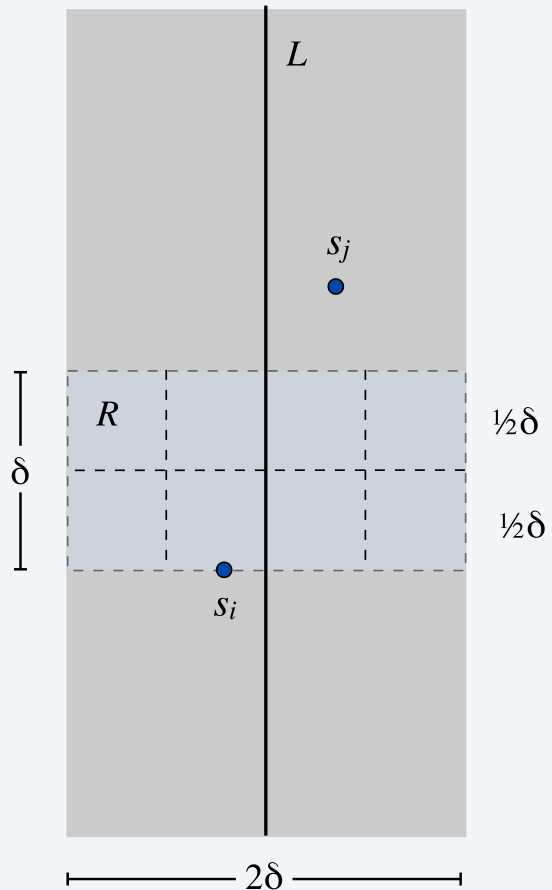
\includegraphics[scale=0.5]{Ln9.image/NearestPointsCpi.png}
    \caption{$C(p_i)$}\label{fig4}
\end{figure}。

接着,我们将这个矩形分拆成左右两个$\delta \times \delta$的正方形,左侧正方形的点集为
$C(p_i)\cap P_1$,右侧正方形的点集为$C(p_i)\cap P_2$,从上述的分治过程可知,这两个点集
内的点之间的距离一定不小于$\delta$。

进一步,我们将$\delta \times \delta$正方形,分拆成四个$\frac{\delta}{2}\times\frac{\delta}{2}$
小正方形,因为这个小正方形的对角线为$\frac{\delta}{\sqrt{2}} < \delta$,所以小正方形中最多
只有一个点,而总共有8个小正方形,最多有8个点,除去$p_i$,则最多只有7个点。

至此,我们完成了父问题的分治与子问题的合并。

\section{分治算法的时间复杂度分析}
首先,第一次排序可以使用时间复杂度为$O(n\log n)$的排序算法,如快速排序或者归并排序。

接着,我们考虑分治过程,即通过分治,我们将规模为$n$的父问题,分为两个规模为$\frac{n}{2}$的子问题。

最后,归并过程中,根据采用的合并策略以及上述对更新操作的证明,我们需要$O(n)$级别的时间完成。

综上,给出递推式如下:

\[
    T(n) = \begin{cases}
        O(1) & 2 \le n \le 3 \\ 
        2T(\frac{n}{2}) + O(n) & n > 3
    \end{cases} 
\]

推导如下:
\begin{align*}
        T(n) &= 2T(\frac{n}{2}) + O(n)\\
             &= 2^2T(\frac{n}{2^2}) + 2O(\frac{n}{2}) + O(n)\\
             &= 2^2T(\frac{n}{2^2}) + 2O(n)\\
             &\vdots \\
             &= 2^k T(\frac{n}{2^k}) + kO(n)\ \ (n = 2 ^ k)\\
             &= O(n) + O(n\log n) \\ 
             &= O(n\log n)
\end{align*}

\section{伪代码}
\begin{algorithm}
    \DontPrintSemicolon{}
    \KwData{
        Point List $P = \{p_i\ \big|\ 1 \le i\le n, p_i = (x_i, y_i)\}$\;
        $P$ should be sorted by x-coordinate in descending order.
    }
    \KwResult{the minimum distance $\delta$}
\Begin{
    \If{$\left| P \right| <= 3$}{ 
        Return the minimum Euclidean-Distance between each pair of points.
    }
    $m \leftarrow \lfloor \frac{n}{2} \rfloor$\;
    $\delta_1 \leftarrow \text{Nearest-Pair}(P[1,\ \ldots,\ m])$\;
    $\delta_2 \leftarrow \text{Nearest-Pair}(P[m + 1,\ \ldots ,\ n])$\;
    $\delta \leftarrow \min \{ \delta_1,\ \delta_2 \}$\;
    $B \leftarrow \text{MergeByY}(P_1,\ P_2)$\;
    \ForEach{$p_i \in B$}{
        \ForEach{$p_j \in C(p_i)$} {
            $\delta \leftarrow \min \{\delta,\ \text{Euclidean-Distance}(p_i, p_j)\}$
        }
    }
    Return $\delta$
}
\caption{Nearest-Pair\label{NPP}}
\end{algorithm}
  \chapter{分治法之大数乘法}
\begin{introduction}
    \item 问题背景
    \item 算法1
    \item 算法2
    \item 伪代码及复杂度分析
\end{introduction}

\section{问题描述}
给定两个大数$A$和$B$, 试计算
\begin{math}
    A * B
\end{math}.
其中$A$和$B$分别表示为
\begin{math}
    A = a_n a_{n-1} a_{n-2} ... a_2 a_1
\end{math}
,
\begin{math}
    B = b_n b_{n-1} b_{n-2} ... b_2 b_1
\end{math}.

\begin{lemma}{“$A + B$”的复杂度}{label_for_a+b}
    计算$A + B$,其复杂度为$O(n)$, 其中$n$为$A$和$B$的十进制位数。
\end{lemma}
\begin{theorem}{“$A * B$”的朴素算法复杂度}{label_for_a*b}
    朴素算法下,将$A$与$B$的各位相乘,再相加各次相乘的结果。
    不难得出,这一过程需要进行$n$次基本乘法与$n+1$次加法。
    根据引理\ref{lem:label_for_a+b},朴素算法下计算$A * B$的时间复杂度为$O(n^2)$.
\end{theorem}
由定理\ref{thm:label_for_a*b}和引理\ref{lem:label_for_a+b}可知,朴素的大数乘法相比加法运算在时间复杂度上高出了一个量级。
由于乘法在计算机中大量存在,我们希望找到更好的算法来降低乘法计算的时间复杂度,以提升计算机的性能。
分治法为我们提供了一条途径。
\section{直接分治法}
\subsection{算法描述}
这是一种简单的分治方法,将两个大数分为前后两部分,进行相乘。不失一般性,这里假设$n$为偶数。将$A$与$B$分割为$A_2$,$A_1$,$B_2$,$B_1$,即:
\begin{displaymath}
    A_2 = a_{n} a_{n-1} ... a_{\frac{n}{2} + 2} a_{\frac{n}{2} + 1}
\end{displaymath}
\begin{displaymath}
    A_1 = a_{\frac{n}{2}} a_{\frac{n}{2} - 1} ... a_2 a_1
\end{displaymath}\\
则$A$被表示为$A = A_2 * 2^{\frac{n}{2}} + A_1$.
同理,$B$可以进行类似的分割,即:
\begin{displaymath}
    B_2 = b_{n} b_{n-1} ... b_{\frac{n}{2} + 2} b_{\frac{n}{2} + 1}
\end{displaymath}
\begin{displaymath}
    B_1 = b_{\frac{n}{2}} b_{\frac{n}{2} - 1} ... b_2 b_1
\end{displaymath}\\
$B$被表示为$B = B_2 * 2^{\frac{n}{2}} + B_1$.\\
对我们的问题而言,计算$A * B$则可以表示为:
\begin{displaymath}
    \begin{split}
        A * B
        & = (A_2 * 2^{\frac{n}{2}} + A_1) * (b_{\frac{n}{2}} b_{\frac{n}{2} - 1} ... b_2 b_1) \\
        & = A_2 B_2 * 2^n + (A_2 B_1 + A_1 B_2) * 2^{\frac{n}{2}} + A_1 B_1
    \end{split}
\end{displaymath}
\begin{algorithm}[H]
    \SetAlgoLined
    \KwData{this text}
    \KwResult{how to write algorithm with \LaTeX2e }
    initialization\;
    \While{not at end of this document}{
        read current\;
        \eIf{understand}{
            go to next section\;
            current section becomes this one\;
        }{
            go back to the beginning of current section\;
        }
    }
    \caption{How to write algorithms}
\end{algorithm}

\bibliography{ref.bib}
\end{document}
